%======================================================================
\chapter{Background}
%======================================================================

\section{Hollow-Core Photonic Crystal Fiber}
\subsection{Conventional TIR Guidance}

\subsection{Bragg Gratings}
\begin{figure}[h!]
	\centering
	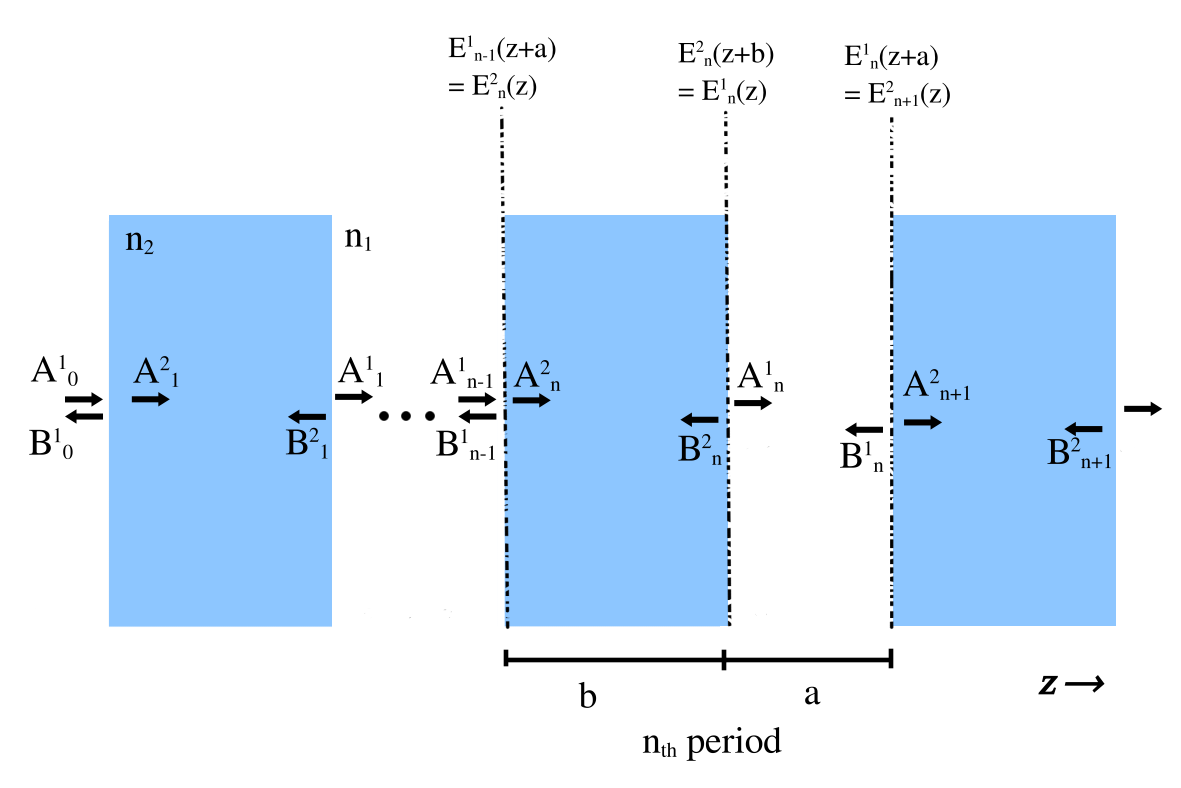
\includegraphics[width=\textwidth]{./Figures/HCPCF/DBR.png}
	\caption{Schematic of quarter wavelength stack}
\end{figure}
\clearpage
\begin{equation}
	\begin{aligned}
		E^1_n(z) &= A^1_n e^{-ik_{z1}(z-(n-1)a)} + B^1_n e^{ik_{z1}(z-(n-1)a)};  (n-1)a+b<z<na\\
		E^2_n(z) &= A^2_n e^{-ik_{z2}(z-(n-1)a)} + B^2_n e^{ik_{z2}(z-(n-1)a)};  (n-1)a<z<(n-1)a+b\\
	\end{aligned}
\end{equation}
Where $k _j= \frac{2\pi}{n_j}$
The boundary conditions:\\
continuous between the layers:
\begin{equation}
		E^1_n(z) = E^2_n(z+b)
\end{equation}
The second condition is that the electric field is smooth, which can be established in the perpendicular magnetic field. Assuming that the electric field is linearly polarized $E(z) = \boldsymbol{\hat{x}}E(z)$, then the magnetic field (via Faraday's law) $H(z) = \boldsymbol{\hat{y}}H(z)$.

\begin{equation}
	\begin{aligned}
		H^1_n(z) &=\frac{1}{\eta_1}[A^1_n e^{-ik_{z1}(z-(n-1)a)} - B^1_n e^{ik_{z1}(z-(n-1)a)}]\\
		H^2_n(z) &= \frac{1}{\eta_2}[A^2_n e^{-ik_{z2}(z-(n-1)a)} - B^2_n e^{ik_{z2}(z-(n-1)a)}]
	\end{aligned}
\end{equation}

\begin{equation}
	\begin{aligned}
			A^2_n(z) = \frac{1}{2}[E^2_n(z) + \eta_2 H^2_n(z)]\\
			B^2_n(z) = \frac{1}{2}[E^2_n(z) - \eta_2 H^2_n(z)]
	\end{aligned}
\end{equation}
Where the impedance $\eta_2 = \frac{\eta_0}{n2}$ \\
Putting these relations into a matrix form we can find a a solution for the transition boundary:
\begin{equation*}
	\begin{aligned}
		\begin{bmatrix}E^1_{n-1}(z+a)\\H^1_{n-1}(z+a) \end{bmatrix} 
		&= \begin{bmatrix}E^2_n(z)\\H^2_n(z) \end{bmatrix}\\
		 \begin{bmatrix}1 & 1\\\eta_1^{-1} & -\eta_1^{-1}\end{bmatrix}\begin{bmatrix}A^1_{n-1}(z+a)\\B^1_{n-1}(z+a) \end{bmatrix}
		 &=\begin{bmatrix}1 & 1\\\eta_2^{-1} & -\eta_2^{-1}\end{bmatrix}\begin{bmatrix}A^2_n(z)\\B^2_n(z) \end{bmatrix} \\
		\begin{bmatrix}A^1_{n-1}(z+a)\\B^1_{n-1}(z+a) \end{bmatrix}
		&= M_{1\rightarrow2}\begin{bmatrix}A^2_n(z)\\B^2_n(z) \end{bmatrix}\\
	\end{aligned}
\end{equation*}

\begin{equation}
	\begin{bmatrix}A^1_{n-1}(z+a)\\B^1_{n-1}(z+a) \end{bmatrix}
	= M_{1\rightarrow2}\begin{bmatrix}A^2_n(z)\\B^2_n(z) \end{bmatrix}\\
\end{equation}

The transition matrix:
\begin{equation}
	M_{1\rightarrow2} = 
	\frac{1}{2}\begin{bmatrix}1+\frac{k_2}{k_1} & 1-\frac{k_2}{k_1}\\1-\frac{k_2}{k_1} & 1+\frac{k_2}{k_1}\end{bmatrix}
\end{equation}

The plane wave propagating though the material will acquire a phase:  
\begin{equation}
	M_{n_2} = \begin{bmatrix}e^{ik_{z2}b} & 0\\0 & e^{-ik_{z2}b}\end{bmatrix}\\
\end{equation}

Thus the travel through the n2 material can be summarized by
\begin{equation}
	\begin{aligned}
		\begin{bmatrix}A^1_{n-1}(z+a)\\B^1_{n-1}(z+a) \end{bmatrix}
		M_{1\rightarrow2}M_{n2}
		\begin{bmatrix}A^2_n(z+b)\\B^2_n(z+b) \end{bmatrix}
	\end{aligned}
\end{equation}

For the electric field through the n1 region :
\begin{equation}
	M_{1\rightarrow2} = 
	\frac{1}{2}\begin{bmatrix}
		1+\frac{k_1}{k_2} & 1-\frac{k_1}{k_2}\\
		1-\frac{k_1}{k_2} & 1+\frac{k_1}{k_2}
	\end{bmatrix}
	\begin{aligned}
		&M_{n_1} =
		\begin{bmatrix}
			e^{ik_{z1}a} & 0\\
			0 & e^{-ik_{z1}a}
		\end{bmatrix}\\
	\end{aligned}
\end{equation}

Becomes one periodic transition matrix:
\begin{equation*}
	M_p = M_{1\rightarrow2}M_{n2}M_{2\rightarrow1}M_{n1} = \begin{bmatrix}m_{11} & m_{12}\\m_{21} & m_{22}\end{bmatrix}\\ 	
\end{equation*}

For an N period block:
\begin{equation*}
	\begin{aligned}
		\begin{bmatrix}A_0\\B_0 \end{bmatrix} 
		&=\frac{1}{2}\begin{bmatrix}1 & \eta_1\\1 & -\eta_1\end{bmatrix} 
		(M_p)^N 
		\begin{bmatrix}1 & \eta_1\\1 & -\eta_1\end{bmatrix}\begin{bmatrix}A_{(N+1)}\\0\end{bmatrix}\\
		\begin{bmatrix}1 \\\eta_1^{-1}\end{bmatrix}A_{(N+1)}
		&= \begin{bmatrix}(-\frac{\eta_2}{\eta_1})^N+(-\frac{\eta_1}{\eta_2})^N \\ (-\frac{\eta_2}{\eta_1})^N-(-\frac{\eta_1}{\eta_2})^N\end{bmatrix}A_{(N+1)}\\
		R &= \Bigg|\frac{(-\frac{\eta_2}{\eta_1})^N-(-\frac{\eta_1}{\eta_2})^N}{(-\frac{\eta_2}{\eta_1})^N+(-\frac{\eta_1}{\eta_2})^N}\Bigg|^2\\
		&=\Bigg|\frac{1-(\frac{\eta_1}{\eta_2})^{2N}}{1+(\frac{\eta_1}{\eta_2})^{2N}}\Bigg|^2; \eta_i = \frac{\eta_0}{\eta_i}, i = 1, 2
	\end{aligned}
\end{equation*}

\subsection{Photonic Crystal Bandgap}
lecture 3


\subsection{Bandgap Shift}
modal magnetic field distributions satisfy:
\begin{equation}
	(\nabla^2_t + k^2n(\boldsymbol{r})^2 - \beta)\boldsymbol{H(r)} = (\nabla_t\times\boldsymbol{H(r)})\times(\nabla_t ln(n(\boldsymbol{r})^2))
\end{equation}
gives scaling law for absolute refractive index at fixed contrast
"a solution for a transverse scale represented by $\Lambda$is replicated in an identical structure with a different $\Lambda$ if the wavelength is scaled proportionately, to keep $k\Lambda$ constant"
Scaling law for the wave equation for the transverse coordinates
$X=x\Lambda^{-1}$ $Y=y\Lambda^{-1}$
where $\Lambda$ is a solution to the transverse scale. 
\begin{equation}
	n(X, Y) = \begin{cases}
		&1, n_1 \text{   (high RI)}\\
		&0, n_2 \text{   (low RI)}
	\end{cases}
\end{equation}
normalized scaled wave equation:
\begin{equation}
	\nabla_\perp^2\Psi + (v^2n(X, Y) - w^2)\Psi = 0
\end{equation}
With $\nabla_\perp = \partial^2/\partial X^2 + \partial^2/\partial Y^2 $
solving for the frequency parameter $v^2$ and eigenvalue $w^2$:
\begin{equation}
	\begin{aligned}
		v^2  &= \Lambda^2k^2(n_1^2 - n_2^2)\\
		w^2 &= \Lambda^2(\beta^2 - k^2n_2^2)
	\end{aligned}
\end{equation}
from the equation above we see that the $w^2$ is determined by the frequency parameter$v^2$ and the index distribution function $n(X, Y)$. This implies that $w^2$ and $v^2$ are invariant with changes to the parameters $k, \Lambda, n_1, n_2$. 
$k = \omega/c$ $\beta = kcos\theta$ longitudinal component of the wavevector. Because the light propagates along the fiber, much of its wavevector is taken up by the longitudinal component. 

In the HCPCF case where the glass refractive index is held constant and the air in the fiber is replaced by a new material the equations can be rewritten with $n1 = n_{glass}$ and $n_2 = n_{air}=1$:
\begin{equation}
	\begin{aligned}
		v^2 - w^2 &= \Lambda^2(k^2n_{glass} - \beta^2)\\
		v &= k\Lambda n_{glass}\sqrt{n_{air} - \frac{n_{air}}{n_{new}}}
	\end{aligned}
\end{equation}
The initial index contrast $N_0 = \frac{n_{air}}{n_{glass}}$ moves to$ N = \frac{n_{new}}{n_{glass}}$ with the change in RI $n_{air} <  n_{new} < n_{glass}$
This leads to the new center bandgap to be governed by the equation: 
\begin{equation}
	\lambda = \lambda_0\sqrt{\frac{1-N^{-2}}{1-N_0^{-2}}}
\end{equation}

"We emphasise that the scalar wave equation (and therefore the scaling laws derived from it) is accurate for the smallest index contrasts only. However, for step-index structures the vector term in Eq. (2) only exists at boundaries, so the scalar wave equation accurately represents wave propagation elsewhere. Since bandgaps arise from interference and resonance effects among such generic waves, the scaling laws of Eq. (5) should be at least approximately valid" ~1.45 RI contrast

\subsection{Mode Distribution}
a) For a two-level atom, the coupling constant -- g -- [Eq. 2.6] scales inversely to this 'effective mode area'  [Eq. before 2.1]  (in the interaction energy term between atom and the field).  mode is like a Gaussian [given by the mode function f(x,y) ] the photon interacts more strongly if the atom is placed in the center of the mode.)\\
effective mode area:
\begin{equation}
	A = \frac{\int dxdy|f_k(x, y)|^2}{|f_k(x_a, y_a)|^2}
\end{equation}
where $f_k(x,y)$ is the transverse mode function and $(x_a,y_a )$ is the position of the atom, is approximately constant in the range of the relevant longitudinal wave numbers\\
coupling constant:
\begin{equation}
	g_\omega = \sqrt{\frac{\omega}{4\pi\epsilon\hbar c A}}d_{eg}
\end{equation}
(2.5) dipole interaction Hamiltonian 

b) Apparently, this coupling constant term tells us parameters such as:\\
i) how likely it is for an excitation in the emitter is released into the waveguide mode $\gamma_{1D}$, versus free-space $\gamma_0$. \cite{mazoni}
\begin{equation}
	\gamma_{1D} = 2\pi g^2_{\omega_A}  = \frac{\sigma_A}{2A}\gamma_0
\end{equation}
"where the second expression directly exhibits the scaling with the transverse extension of the waveguide. It is related to the atomic radiative cross section $\sigma_A = \frac{3\lambda^2}{2\pi}$. A natural lower bound on the transverse mode size is at about $A \sim (\frac{\lambda}{2})^2$. (lowest-order mode in hollow metallic wave- guide), implying a maximum achievable coupling ratio $\gamma_{1D}/\gamma_0 \sim 1$. In the range $\sigma_A \sim A$, one has a strong waveguide-atom coupling, which is manifested by the fact that the atom dissipates its energy equally into the waveguide and the free-space ‘‘lossy’’ modes."\cite{domokos}

ii) optical depth (OD) for a single atom is (about) the ratio of $ (\gamma_{1D})/ (\gamma_{0})$ or the ratio of the cross-section area of the atom to that of the effective mode-area. 
\begin{equation}
 	OD = \frac{\sigma_A}{\sigma_M} = \frac{\gamma_{1D}}{\gamma_0}
\end{equation}

c) OPTICAL DEPTH CALCULATIONS: Optical depth (OD) tells about how opaque the system is. Transmitted intensity goes by $T = exp(-OD)$. Normally, N emitters might scale linearly to give an optical depth ~$N*OD$. But now (due to its position) each emitter might have its own mode area.\\

Examples of taking this into account (with maybe slightly different conventions) for atoms are mentioned in these two references\cite{bajcsy, hilton}: 
\begin{equation}
	OD_{fiber} = \int^L_0 \int^{r}_0 n(\rho, z) OD 2\pi \rho d\rho dL
\end{equation}
$r$ and $L$ represent the radius and length of the ensemble, which in the case of solution-filled HCPCF is the radius and length of the fiber. This assumes that the particulates outside of the core do not have a significant contribution. 

\begin{thebibliography}{hcpcf}
	\bibitem{domokos} P. Domokos, P. Horak, and H. Ritsch, “Quantum description of light-pulse scattering on a single atom in waveguides,” Phys. Rev. A, vol. 65, no. 3, p. 033832, Mar. 2002, doi: 10.1103/PhysRevA.65.033832.
	
	\bibitem{solano} P. Solano et al., “Optical Nanofibers: a new platform for quantum optics,” vol. 66, 2017, pp. 439–505. doi: 10.1016/bs.aamop.2017.02.003.\\
	
	\bibitem{mazoni} M. T. Manzoni, “New Systems for Quantum Nonlinear Optics,”. 2017, Thesis, p. 39-40.
	
	\bibitem{bajcsy} M. Bajcsy et al., “Laser-cooled atoms inside a hollow-core photonic-crystal fiber,” Phys. Rev. A, vol. 83, no. 6, p. 063830, Jun. 2011, doi: 10.1103/PhysRevA.83.063830. \\
	\bibitem{hilton} A. P. Hilton, C. Perrella, F. Benabid, B. M. Sparkes, A. N. Luiten, and P. S. Light, “High-efficiency cold-atom transport into a waveguide trap,” Phys. Rev. Applied, vol. 10, no. 4, p. 044034, Oct. 2018, doi: 10.1103/PhysRevApplied.10.044034. A
\end{thebibliography}